\documentclass[10pt]{article}
% Change "article" to "report" to get rid of page number on title page
\usepackage{amsmath,amsfonts,amsthm,amssymb}
\usepackage{setspace}
\usepackage{graphicx,float,wrapfig}
%\usepackage{parskip}
\usepackage{enumerate}

\usepackage{fourier}
\usepackage[T1]{fontenc}
\usepackage[protrusion=true,expansion=true]{microtype}


\usepackage{tikz} % For drawing diagrams
\usetikzlibrary{calc}
\tikzset{
% Two node styles for game trees: solid and hollow
solid node/.style={circle,draw,inner sep=1.5,fill=black},
hollow node/.style={circle,draw,inner sep=1.5}
}

% In case you need to adjust margins:
\topmargin=-0.45in      %
\evensidemargin=0in     %
\oddsidemargin=0in      %
\textwidth=6.5in        %
\textheight=9.0in       %
\headsep=0.25in         %
\parindent=0in

\usepackage[nodayofweek]{datetime} \usdate
% Pdf metadata
\pdfinfo{  /Author (Blake Riley)
           /Title (Econ 502 Handout 2)
           /Keywords ()
           /ModDate (D:\pdfdate)}

\newtheoremstyle{basic}% name
   {5pt}% Space above
   {5pt}% Space below
   {\itshape \leftskip=1em}% Body font
   {-1em}% Indent amount
   {\bfseries}% Theorem head font
   {:}% Punctuation after theorem head
   { }% Space after theorem head
   {}% Theorem head spec (can be left empty, meaning `normal')
\theoremstyle{basic}
\newtheorem{exercise}{Exercise}[]
\newtheorem{definition}{Definition}[section]
\newtheorem{theorem}{Theorem}[section]
\newtheorem{lemma}[theorem]{Lemma}


%%%%%%%%%%%%%%%%%%%%%%%%%%%%%%%%%%%%%%%%%%%%%%%%%%%%%%%%%%%%

% Custom commands

\newcommand{\R}{\mathbb{R}}
\newcommand{\N}{\mathbb{N}}
\newcommand{\E}{\operatorname{E}}
\renewcommand{\P}{\operatorname{Pr}}
\newcommand{\Var}{\operatorname{Var}}
\newcommand{\Cov}{\operatorname{Cov}}
\newcommand{\cond}{\,|\,}
\newcommand{\bigcond}{\;\big|\;}
\newcommand{\argmax}{\mathop{\operatorname{arg\,max}}}
\newcommand{\noti}{{{\scriptscriptstyle-}\!i}}
\newcommand{\notj}{{{\scriptscriptstyle-}\!j}}
\newcommand{\notij}{{{\scriptscriptstyle-}\!\{i,j\}}}
\newcommand{\I}{\mathbb{I}}

%%%%%%%%%%%%%%%%%%%%%%%%%%%%%%%%%%%%%%%%%%%%%%%%%%%%%%%%%%%%%
%%%%%%%%%% The main document content
%%%%%%%%%%%%%%%%%%%%%%%%%%%%%%%%%%%%%%%%%%%%%%%%%%%%%%%%%%%%%

\begin{document}
\begin{spacing}{1.0}

\noindent
\textbf{Handout 2} \\
Econ 533 \\
February 5, 2016 \\
TA: Blake Riley \\

\begin{center}
{\Large Microeconomic Theory II: Spring 2016}
\end{center}

\section{Refinements in dynamic games}

\subsection{Subgame perfect Nash equilibria}

\begin{definition}
  A \textbf{subgame} of an extensive form game is a subset of the
  game having the following properties:
  \begin{itemize}
  \item It begins with an information set containing a
    single node (since games start from a single node).
  \item It contains all the nodes that are successors of
    this node and only these nodes.
  \item If a node is in the subgame, then all nodes in
    the same information set are in the subgame (we can't
    cut through information sets).
  \end{itemize}
\end{definition}

\begin{definition}
  A strategy profile $\sigma = (\sigma_1, \ldots, \sigma_N)$ in an
  extensive form game is a \textbf{subgame perfect Nash equilibrium (SPNE)}
  of this game if it induces a Nash equilibrium in every subgame of the
  game.
\end{definition}

Every SPNE is a NE, but not vice versa (which is why it's known as a
refinement). If the only subgame of an extensive form game is the game
itself, then every NE is a SPNE.

\subsection{Identifying SPNEs}

Backward induction:

\begin{enumerate}
\item Identify how many subgames you have. If the only subgame is the game
  itself, every NE is an SPNE. In simple cases, drawing the normal form and
  finding NE is the best route. If this is applicable, stop here.
\item Go to the final subgames and find the NE of the final subgames.
\item Pick one of the equilibria and replace the final subgames by the
  corresponding equilibrium payoff vectors.
\item Now start the recursion. Do the previous steps again for the reduced
  game. If you find multiple equilibria at any step, each of the possible
  combinations constitutes a SPNE.
\item If there is a unique equilibrium strategy for each player at each
  possible subgame, the SPNE is unique.
\end{enumerate}

\begin{lemma}
  In a finite extensive form game, if no player has the same payoffs at any
  two terminal nodes, there is a unique Nash equilibrium that can be
  derived by backward induction. This is then also the unique SPNE.
\end{lemma}

\subsection{Weak perfect Bayesian Nash equilibria}

\begin{definition}
  A profile of strategies and systems of beliefs $(\sigma, \mu)$ is a
  \textbf{weak perfect Bayesian Nash equilibrium (WPBE)} in an extensive
  form game if it has the following properties:
  \begin{itemize}
  \item The strategy profile $\sigma$ is sequentially rational given given
    belief system $\mu$, i.e. once an information set is reached on the
    equilibrium path, no player finds it worthwhile to revise his strategy.
  \item The systems of beliefs $\mu$ is derived from strategy profile
    $\sigma$ using Bayes rule whenever possible.
  \end{itemize}
\end{definition}

The probability of being at one specific node in an information set that
lies on the equilibrium path has to be derived by Bayes rule. Notice
however, we don't put any restrictions on how to derive beliefs for
information sets not on the equilibrium path. All WPBE are NE, but not vice versa.

\subsection{How to identify WPBEs}

\begin{enumerate}
\item Check whether each player has some dominant strategies. This can save
  a significant amount of time.
\item Assign general beliefs to each node with non-singleton information
  sets and apply ``sequential rationality,'' i.e. compute expected payoffs
  of each possible action at this information set using the general
  beliefs. Find out which action has the higher expected payoff for which
  threshold beliefs. You will probably have several cases.
\item Apply sequential rationality to each singleton information set given
  the cases of the other information sets.
\item Update the beliefs that are on the equilibrium paths and ensure
  consistency with the assumed beliefs from step 2.
\end{enumerate}

\subsection{Sequential equilibria}

\begin{definition}
  A profile of strategies and systems of belief $(\sigma, \mu)$ is a
  \textbf{sequential equilibrium} (denoted elsewhere, perhaps more
  consistently, as \textbf{perfect Bayesian equilibria}) in an extensive
  form game if it has the following properties:
  \begin{itemize}
  \item The strategy profile $\sigma$ is sequentially rational given belief
    system $\mu$.
  \item There exists a sequence of completely mixed strategies
    $\left\{\sigma^k\right\}_{k=1}^\infty$ with $\lim_{k \to \infty} \sigma^k =
    \sigma$ such that $\mu = \lim_{k \to \infty} \mu^k$, where $\mu^k$ denotes
    the beliefs derives from strategy profile $\sigma^k$ using Bayes rule.
  \end{itemize}
\end{definition}

Sequential equilibria are WPBE and SPNE.

\subsection{Identifying sequential equilibria}

\begin{enumerate}
\item First you have to identify all WPBEs. If there is a unique WPBE and
  all information sets of all players are on the equilibrium path, then it
  is also a sequential equilibrium.
\item If not all information sets are reached: try constructing a sequence
  of mixed strategies that converge to the equilibrium strategies so that
  the induced beliefs converge to the beliefs given by the WPBE. If you
  find one such sequence you are done.
\item Showing that something is not a sequential equilibrium can be
  difficult using the sequence approach. You would have to prove that for
  every sequence of mixed strategies, the induced beliefs don't converge to
  the proposed beliefs. A better approach: try to show it's not a
  SPNE. If this is the case, then it can't be a sequential equilibrium.
\end{enumerate}

\subsection{Tips}

\begin{itemize}
\item Every sequential equilibrium is a WPBE and a SPNE.
\item Not every WPBE is a SPNE.
\item Finding a single sequence that does not converge to a pair $(\sigma,
  \mu)$ is not enough to show this is not a sequential equilibrium!
\item If for a pair $(\sigma, \mu)$ every information set is reached and
  $(\sigma, \mu)$ is a WPBE, then it is also a sequential equilibrium (and
  hence also a SPNE).
\item If you show that $(\sigma, \mu)$ is a WPBE, but not a SPNE, then it
  is not a sequential equilibrium.
\end{itemize}

\newpage
\section{Exercises}

\begin{exercise}
  If a player has $N$ information sets with $m_i$ choices at the $i$-th, how many
  strategies does that player have?
\end{exercise}

\begin{exercise}
  Find all the SPNEs and WPNEs:
  \begin{center}
    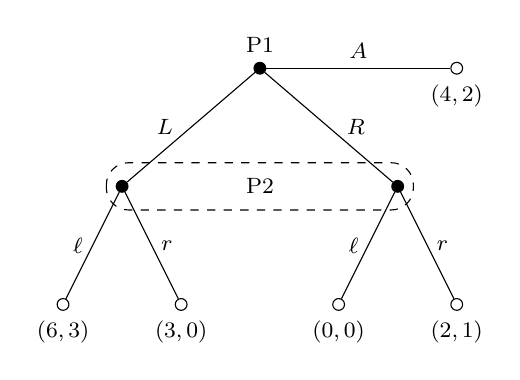
\begin{tikzpicture}[scale=1,font=\footnotesize]
      % Specify spacing for each level of the tree
      \tikzstyle{level 1}=[level distance=15mm,sibling distance=35mm]
      \tikzstyle{level 2}=[level distance=15mm,sibling distance=15mm]
      % The Tree
      \node(0)[solid node,label=above:{P1}]{}
      child[missing] % Missing very left node to balance tree
      % Actual left node
      child{node(1)[solid node]{} child{node[hollow node,label=below:{$(6,3)$}]{}
          edge from parent node[left]{$\ell$} } child{node[hollow
          node,label=below:{$(3,0)$}]{} edge from parent node[right]{$r$} } edge from
        parent node[left,xshift=-3]{$L$} }
      % Right node
      child{node(2)[solid node]{} child{node[hollow node,label=below:{$(0,0)$}]{}
          edge from parent node[left]{$\ell$} coordinate[pos=.8] (l)}
        child{node[hollow node,label=below:{$(2,1)$}]{} edge from parent
          node[right]{$r$} coordinate[pos=.8] (r)} edge from parent
        node[right,xshift=3]{$R$} } child[grow=right, level distance = 25mm]{
        node[hollow node, label=below:{$(4,2)$}]{} edge from parent node[above]{$A$}
      } ;
      % information set
      \draw[dashed,rounded corners=8]($(1) + (-.2,.3)$)rectangle($(2) +(.2,-.3)$);
      % specify mover at 2nd information set
      \node at ($(1)!.5!(2)$) {P2};
    \end{tikzpicture}
  \end{center}
\end{exercise}

\begin{exercise} Consider the following game tree:
  \begin{center}
      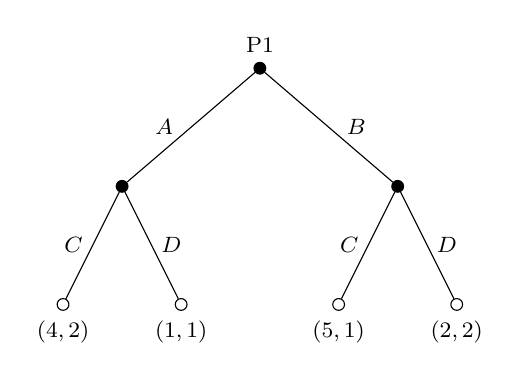
\begin{tikzpicture}[scale=1,font=\footnotesize]
        % Specify spacing for each level of the tree
        \tikzstyle{level 1}=[level distance=15mm,sibling distance=35mm]
        \tikzstyle{level 2}=[level distance=15mm,sibling distance=15mm]
        % The Tree
        \node(0)[solid node,label=above:{P1}]{}
        child{node(1)[solid node]{}
          child{node[hollow node,label=below:{$(4,2)$}]{}
            edge from parent node[left]{$C$} }
          child{node[hollow node,label=below:{$(1,1)$}]{}
            edge from parent node[right]{$D$} }
          edge from parent node[left,xshift=-3]{$A$}
        }
        child{node(2)[solid node]{}
          child{node[hollow node,label=below:{$(5,1)$}]{}
            edge from parent node[left]{$C$}}
          child{node[hollow node,label=below:{$(2,2)$}]{}
            edge from parent node[right]{$D$}}
          edge from parent node[right,xshift=3]{$B$}
        };
        %%% uncomment to draw information set
        % \draw[dashed,rounded corners=10]($(1) +
        % (-.2,.25)$)rectangle($(2) +(.2,-.25)$);
        % % specify mover at 2nd information set
        % \node at ($(1)!.5!(2)$) {$P2$};
      \end{tikzpicture}
    \end{center} 
  \begin{enumerate}
  \item How many SPNEs are there in this game? Are there other Nash equilibria in
    pure strategies?
  \item Suppose player two cannot observe player one's move. What is the new
    extensive form? What are the Nash equilibria?
  \item Suppose player two observes correctly with probability $p \in (0,1)$ and
    incorrectly with probability $1-p$ where $p$ is common knowledge. What is the
    extensive form? What is the set of WPNEs (in pure strategies)?    
  \end{enumerate}  
\end{exercise}

\begin{exercise}[Ultimatum Game] Player one chooses an amount $x \in [0,1]$ which
  player two has the option to accept or reject. What are the SPNEs of this game?
  \begin{center}
    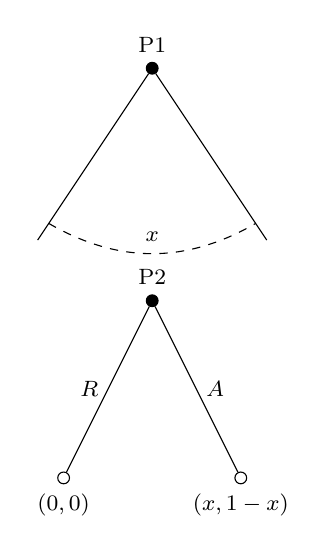
\begin{tikzpicture}[scale=1.5,font=\footnotesize]
      % Specify spacing for each level of the tree
      \tikzstyle{level 1}=[level distance=15mm,sibling distance=10mm]
      \tikzstyle{level 2}=[level distance=15mm,sibling distance=15mm]
      % The Tree
      \node(head)[solid node, label=above:{P1}]{}
      % Left branch with invisible node
      child{node[solid node, white]{} edge from parent coordinate[pos=.9] (lbranch)}
      % Middle branch
      child{ node[yshift=3]{$x$} % Add label for arc
        node[solid node, yshift=-20, label=above:{P2}]{} child{node[hollow
          node,label=below:{$(0,0)$}]{} edge from parent node[left]{$R$}}
        child{node[hollow node,label=below:{$(x,1-x)$}]{} edge from parent
          node[right]{$A$}} edge from parent
        [draw=none] % Hide edge from head to middle branch
      }
      % Right branch with hidden node
      child{node[solid node, white]{} edge from parent coordinate[pos=.9] (rbranch)}
      ;
      % Draw arc
      \draw[dashed,bend right] (lbranch) to (rbranch);
    \end{tikzpicture}
  \end{center}  
\end{exercise}






%%%%%%%%%%%%%%%
\end{spacing}
\end{document}
%%%%% FIN %%%%%
%%%%%%%%%%%%%%%